%%%%%%%%%%%%%%%%%%%%%%%%%%%%%%%%%%%%%%%%%%%%%%%%%
% ACOSUS Paper: An AI-driven Transfer Student Advising System
% Document Class: Article with ACM-style formatting
%%%%%%%%%%%%%%%%%%%%%%%%%%%%%%%%%%%%%%%%%%%%%%%%%

\documentclass[a4paper,10.5pt,twoside]{article}
\hyphenpenalty=500
\tolerance=1000
\emergencystretch=3em
\textwidth=125mm
\textheight=200mm
\usepackage[top=3cm, bottom=3cm, inner=3cm, outer=3cm, includehead]{geometry}
\usepackage{fancyhdr}
\pagestyle{fancy}
\fancyhead{}
\fancyfoot{}
\raggedbottom
\usepackage{xurl}
\usepackage{graphicx}
\usepackage{alltt}
\usepackage{amsmath}
\usepackage{booktabs}
\usepackage[hidelinks, pdftex]{hyperref}
\usepackage{float}

% TikZ packages for diagrams
\usepackage{tikz}
\usetikzlibrary{shapes.geometric, arrows.meta, positioning, fit, backgrounds, calc}

% Define colors for diagrams
\definecolor{targetsurvey}{HTML}{FFF3E0}
\definecolor{factorsurvey}{HTML}{E3F2FD}
\definecolor{processing}{HTML}{F3E5F5}
\definecolor{outputgreen}{HTML}{E8F5E9}
\definecolor{stage1green}{HTML}{D4EDDA}
\definecolor{stage1border}{HTML}{28A745}
\definecolor{stage2yellow}{HTML}{FFF3CD}
\definecolor{stage2border}{HTML}{FFC107}
\definecolor{stage3blue}{HTML}{CCE5FF}
\definecolor{stage3border}{HTML}{007BFF}
\definecolor{framegray}{HTML}{F8F9FA}
\definecolor{frameborder}{HTML}{6C757D}
\definecolor{modelpink}{HTML}{FCE4EC}
% Colors for fig2 (Three-Stage Pipeline)
\definecolor{stage1}{RGB}{76,175,80}
\definecolor{stage2}{RGB}{255,152,0}
\definecolor{stage3}{RGB}{100,149,237}
\definecolor{inputred}{RGB}{183,28,28}
\definecolor{outputviolet}{RGB}{103,58,183}
\definecolor{pipelineborder}{RGB}{120,60,60}
% Colors for fig3 (Survey Processing)
\definecolor{surveyblue}{RGB}{66,133,244}
\definecolor{surveyboxfill}{RGB}{215,232,252}
\definecolor{processorange}{RGB}{234,67,53}
\definecolor{processboxfill}{RGB}{253,232,226}
\definecolor{processboxborder}{RGB}{230,150,100}
\definecolor{modelgreen}{RGB}{15,100,80}
\definecolor{modelboxfill}{RGB}{200,230,225}
\definecolor{modelboxborder}{RGB}{100,180,170}
% Colors for fig4 (System Architecture)
\definecolor{dblue}{RGB}{60,100,180}

% TikZ styles
\tikzset{
    surveybox/.style={rectangle, rounded corners=3pt, minimum width=2.2cm, minimum height=0.8cm, text centered, draw=black!60, font=\scriptsize, text width=2cm, align=center},
    groupbox/.style={rectangle, rounded corners=5pt, draw=black!40, thick},
    arrow/.style={-{Stealth[length=2mm]}, thick, black!70},
    dashedarrow/.style={-{Stealth[length=2mm]}, thick, black!50, dashed},
    stagebox/.style={rectangle, rounded corners=5pt, minimum width=3cm, minimum height=1.8cm, draw, thick, text width=2.8cm, align=center, font=\scriptsize},
    layerbox/.style={rectangle, rounded corners=3pt, minimum width=2cm, minimum height=0.6cm, text centered, draw=black!60, font=\tiny, text width=1.8cm, align=center},
}
\urlstyle{same}
\usepackage[T1]{fontenc}
\usepackage[utf8]{inputenc}
\usepackage{lmodern}
\usepackage{csquotes}
\usepackage[style=numeric, backend=biber, sorting=none]{biblatex}
\addbibresource{references.bib}
\pagenumbering{arabic}
\setcounter{page}{1}

\usepackage[english]{babel}

\begin{document}
\fancyhead[LE]{\thepage\ \ \ \ [Author Last Names]}
\fancyhead[RO]{ACOSUS: AI-driven Transfer Student Advising\ \ \ \ \thepage}

\begin{center}
\LARGE
\textbf{An AI-driven Transfer Student Advising System: Design, Implementation, and Evaluation}\\[12pt]
\normalsize
\textbf{Author1,\footnote{Author1 title, Author1 institution, Author1 country, Author1 email.} Author2,\footnote{Author2 title, Author2 institution, Author2 country, Author2 email.} and Author3\footnote{Author3 title, Author3 institution, Author3 country, Author3 email.}}\\[4pt]
\end{center}

\begin{abstract}
\normalsize
Transfer students---particularly those from underrepresented backgrounds in computing---face unique challenges that traditional advising systems fail to address: fragmented information across institutions, limited visibility into pre-transfer trajectories, and predictive models calibrated on native student populations. We present ACOSUS (AI-driven Counseling System for Underrepresented Students), an intelligent advising platform designed specifically for transfer student populations. The system introduces two architectural innovations: a dual-survey architecture that separates outcome measurement from feature collection while providing advisors with unified student profiles, and a progressive learning framework that treats data scarcity as a fundamental design constraint rather than a limitation to overcome. A pilot evaluation with transfer students at a public urban university validated the data collection workflow, with participants rating both Perceived Ease of Use and Perceived Usefulness highly. The system is currently operational and collecting observations to enable future evaluation of its predictive capabilities.\vskip 2mm
\textbf{Keywords:} transfer students, intelligent advising, machine learning, higher education, student success prediction.
\end{abstract}

%%%%%%%%%%%%%%%%%%%%%%%%%%%%%%%%%%%%%%%%%%%%%%%%%
% SECTION 1: INTRODUCTION
%%%%%%%%%%%%%%%%%%%%%%%%%%%%%%%%%%%%%%%%%%%%%%%%%
\section{Introduction}\label{sec:introduction}

In recent years, an alternative pathway to baccalaureate attainment has gained prominence: a substantial share of students now begin their post-secondary careers in community colleges and later transfer to four-year universities to complete their degrees. National studies estimate that more than one-third of all undergraduates follow this route \cite{ishitani2018student,roksa2008credits}, with the proportion even higher in computing and other STEM majors and among first-generation, low-income, and racially minoritized learners \cite{wali2025transfer,computingtransfer2024,jabbar2019complex}. Although the transfer pathway offers an affordable on-ramp to bachelor's-level credentials \cite{socialcognitive2022,factoranalysis2023}, community colleges and destination universities face significant challenges in coordinating policies and support services for this population \cite{topicmodeling2024,factoranalysis2023}. Advisors on both campuses must navigate opaque articulation agreements, uneven credit recognition, and limited visibility into students' prior coursework \cite{nguyen2024community,roksa2008credits,preposttransfer2014}. The task is further complicated for students from groups traditionally under-represented in STEM, who must contend simultaneously with structural barriers, financial constraints, and feelings of isolation in new academic and social environments \cite{computingtransfer2024,wang2020road,socialcognitive2022}.

Persistence and timely graduation are therefore central concerns. Transfer students are more likely than native students to experience ``transfer shock,'' a transient decline in GPA and sense of belonging during their first two semesters after matriculation \cite{jaggars2025,laanan2010adjustment}, and they exhibit higher attrition rates overall. Prior quantitative research has identified a set of structured indicators---cumulative GPA, number of credits accepted, standardized-test scores, distance between sending and receiving institutions, and availability of financial aid---that correlate with retention and completion \cite{wang2020road,factoranalysis2023,jaggars2025,thiry2023,townsend2009}. Yet these metrics, while informative, paint an incomplete picture \cite{topicmodeling2024,socialcognitive2022}. Qualitative studies have repeatedly emphasized the importance of social support, faculty mentorship, and campus engagement opportunities such as research assistantships or hackathons, factors that are difficult to capture in traditional student-information systems \cite{topicmodeling2024,thiry2023}.

Effective advising is widely regarded as the linchpin of transfer-student success \cite{topicmodeling2024,preposttransfer2014,lukszo2020,thiry2023}. Students expect clear, timely, and individualized guidance, but caseloads at many institutions leave advisors little time to drill into each learner's unique background, ambitions, and constraints \cite{topicmodeling2024,preposttransfer2014}. Existing advising dashboards largely replicate registrar data and early-alert metrics designed for native cohorts; they rarely incorporate pre-transfer trajectories, articulation nuances, or unstructured signals such as students' own narratives of their decision-making processes \cite{nguyen2024community,preposttransfer2014}. Consequently, predictive models can misclassify risk and amplify equity gaps \cite{computingtransfer2024,socialcognitive2022}. A more holistic, data-rich approach---one that blends quantitative indicators with the lived experiences of transfer students---is urgently needed \cite{topicmodeling2024,socialcognitive2022}.

To address this gap, we designed and evaluated an intelligent advising system that merges academic records with social-cognitive, financial, and experiential data collected both before and after transfer. Our contributions are as follows:

\begin{enumerate}
    \item We introduced the first intelligent advising platform designed specifically for transfer students, integrating standard academic records with student-provided background to build a unified longitudinal profile.
    \item We developed a dual-survey architecture that separates outcome measurement (Target Surveys) from feature collection (Factor Surveys), enabling systematic capture of transfer-specific variables---academic background, financial circumstances, and logistical constraints---while providing advisors with unified, structured student profiles through a centralized dashboard.
    \item We implemented a modular prediction architecture with extensive configuration support that enables adaptation to diverse institutional contexts and emerging methodological advances. The system's algorithm-agnostic design—where any compatible method can serve each pipeline stage—allows researchers to empirically evaluate alternative approaches on their specific transfer student populations, while configuration options for survey linkage, phase transitions, and hyperparameters support customization without code modification.
    \item We validated the platform through a pilot deployment with transfer students, who provided feedback on their experience using it, showing that it streamlines self-advising workflows and is perceived as trustworthy, actionable, and equity-enhancing.
\end{enumerate}

The remainder of the paper is organized as follows. Section~\ref{sec:literature} reviews related work on transfer-student success and intelligent advising. Section~\ref{sec:design} describes our system design and methodology. Section~\ref{sec:implementation} presents implementation details. Section~\ref{sec:evaluation} reports empirical findings from our pilot study. Section~\ref{sec:conclusion} concludes and outlines directions for future research.

%%%%%%%%%%%%%%%%%%%%%%%%%%%%%%%%%%%%%%%%%%%%%%%%%
% SECTION 2: LITERATURE REVIEW
%%%%%%%%%%%%%%%%%%%%%%%%%%%%%%%%%%%%%%%%%%%%%%%%%
\section{Literature Review}\label{sec:literature}

The growing body of work on transfer-student outcomes can be grouped into two complementary strands \cite{factoranalysis2023}. The first investigates personal and academic characteristics that shape the transfer journey; the second examines institutional practices---especially advising---that mediate these effects.

Early conceptual models, notably Ty et al.'s adaptation of Social-Cognitive Career Theory, frame upward transfer as a function of ``person inputs'' (e.g., socioeconomic status, self-efficacy) and ``transfer receptivity,'' a campus-level construct encompassing articulation policies and support services \cite{computingtransfer2024}. Empirical validation across STEM programs shows that self-efficacy and goal-setting scores tend to rise after students move to four-year university, even as they confront unfamiliar academic norms \cite{socialcognitive2022,topicmodeling2024}. Quantitative factor-analysis studies corroborate the salience of financial considerations, institutional reputation, geographic proximity, and family expectations in the initial decision to transfer \cite{factoranalysis2023}, while regression analyses link post-transfer GPA to race/ethnicity and first-generation status \cite{computingtransfer2024}. Topic-modeling of open-ended survey and social-media data adds texture to this portrait, revealing frustration with credit evaluation, heavy commuting burdens, and limited on-campus engagement opportunities \cite{topicmodeling2024}.

Advising research converges on the notion of ``transfer student capital,'' the knowledge and networks students accrue as they navigate multiple institutions \cite{laanan2010adjustment,lukszo2020}. When formal channels fall short, many seek guidance on Reddit, Discord, or peer-run forums, especially about financial aid, housing, and course selection \cite{topicmodeling2024,nguyen2024community}. Qualitative interviews highlight how relationship-rich advising mitigates transfer shock and fosters a sense of belonging \cite{thiry2023,jaggars2025}. Yet advisors themselves report difficulty keeping abreast of ever-shifting articulation rules and program maps, given heavy caseloads \cite{preposttransfer2014,nguyen2024community}.

Technology-mediated solutions have begun to emerge, but most commercial platforms were designed for native student populations \cite{nguyen2024community}. Predictive-analytics tools typically ingest registrar feeds and LMS (Learning Management Systems) clickstreams, rarely accounting for variables such as credit-completion velocity or social-belonging indicators that matter disproportionately for transfer cohorts \cite{nguyen2024community,topicmodeling2024}. Reviews warn that models calibrated on homogeneous populations risk biased predictions and may inadvertently disadvantage students from minoritized backgrounds \cite{socialcognitive2022,computingtransfer2024}. Only a handful of prototype systems explicitly target transfer populations, and these remain at pilot scale \cite{topicmodeling2024,socialcognitive2022}.

Against this backdrop, scholars have called for mixed-methods approaches that integrate quantitative data with rich qualitative insights \cite{socialcognitive2022,wang2020road}. Topic modeling offers a promising avenue: by extracting latent themes from narrative responses, researchers can surface under-documented challenges and aspirations. Deng et al.\ applied Revealed Causal Mapping to narrative survey responses to trace how social media use shapes the academic experiences and social capital of first-generation learners \cite{deng2021}, while Thiry et al.\ leveraged mixed-methods case studies to develop strategic frameworks for STEM transfer support \cite{thiry2023}. However, few studies have fed such unstructured insights back into automated advising tools.

A related but distinct challenge compounds the technology gap: even where transfer-specific systems might be developed, data scarcity constrains their effectiveness. Paradoxically, this scarcity stems not from a shortage of transfer students but from systemic information fragmentation across institutional boundaries \cite{nguyen2024community,roksa2008credits}. When students transfer, only a narrow slice of their academic record---credits earned, GPA, and course equivalencies---moves with them; the rich contextual understanding that community college advisors accumulate over semesters of interaction rarely transfers \cite{roksa2008credits,nguyen2024community}. Factors such as family obligations, financial stressors, career motivations, and early warning signs identified by sending-institution advisors remain undocumented or siloed in systems inaccessible to the receiving university \cite{preposttransfer2014,topicmodeling2024}. University advisors must therefore reconstruct this understanding through time-intensive intake conversations, and machine learning systems face a cold-start problem at the institutional level: each university must build its training corpus from scratch, accumulating labeled observations one student at a time \cite{coleman2019coldstart}. Traditional predictive approaches face cold-start challenges in small-cohort settings \cite{coleman2019coldstart}---and when the very factors most predictive of success are precisely what the transfer process fails to preserve \cite{socialcognitive2022,roksa2008credits}.

The present work answers these gaps from a systems perspective. Drawing on prior quantitative and qualitative insights, we engineer an integrated advising platform that fuses standard academic records (e.g., transfer-credit counts, GPA history, enrollment status) with student-supplied experience data and applies a lightweight, interpretable classifier to generate individualized success forecasts. An intuitive dashboard delivers these forecasts directly to students. Initial user feedback from the pilot indicates that the system fills a critical void in current transfer-student support practices and offers a scalable template for institutions seeking to improve equity and retention.

%%%%%%%%%%%%%%%%%%%%%%%%%%%%%%%%%%%%%%%%%%%%%%%%%
% SECTION 3: SYSTEM DESIGN AND METHODOLOGY
%%%%%%%%%%%%%%%%%%%%%%%%%%%%%%%%%%%%%%%%%%%%%%%%%
\section{System Design and Methodology}\label{sec:design}

To address the data constraints and advising challenges outlined in Section~\ref{sec:introduction}, we designed ACOSUS (AI-driven Counseling System for Underrepresented Students). This section presents the system's core architectural innovations: a dual-survey architecture that captures transfer-specific variables while supporting advisor workflows (\S\ref{subsec:dualsurvey}), and a progressive learning framework designed for the small-data regime inherent in departmental-level or institutional level transfer advising (\S\ref{subsec:progressive}).

\subsection{The Dual-Survey Architecture}\label{subsec:dualsurvey}

Before proceeding, we clarify terminology used throughout this paper. ACOSUS frames transfer student success prediction as a supervised learning problem where the goal is to predict an outcome from a set of input variables. We use the following terms interchangeably based on context:

\begin{itemize}
    \item \textbf{Target Survey / Outcome ($Y$)}: The survey instrument that measures what we want to predict---the student's likelihood of academic success. In machine learning terminology, this is the \emph{label} or \emph{dependent variable}.
    \item \textbf{Factor Survey / Predictors ($X$)}: The survey instruments that collect information used to make predictions---academic background, financial circumstances, and logistical constraints. In machine learning terminology, these are \emph{features} or \emph{independent variables}.
    \item \textbf{Constructs}: Psychological or educational concepts (e.g., self-efficacy, institutional commitment) that we operationalize through survey questions. A single Factor Survey may measure multiple constructs.
\end{itemize}

The variables most predictive of transfer success---credit articulation outcomes, ``transfer shock'' severity, belonging uncertainty, and financial precarity---are seldom captured in standard institutional systems \cite{topicmodeling2024,computingtransfer2024,socialcognitive2022}. Furthermore, academic advisors lack unified access to the information they need; prior research documents that advisors spend significant time gathering student data from disparate sources before providing meaningful guidance \cite{preposttransfer2014,thiry2023}. ACOSUS addresses both challenges through a Dual-Survey Architecture that simultaneously feeds AI models and consolidates advisor-facing information.

Prior research on transfer student success has identified multiple dimensions that contribute to successful degree completion, including academic self-efficacy, institutional commitment, social integration, and career goal clarity \cite{factoranalysis2023,topicmodeling2024,computingtransfer2024}. Our earlier factor analysis work identified clusters of social-cognitive variables---academic confidence, time management, financial stability, and support systems---that distinguish successful transfer students from those who struggle \cite{factoranalysis2023}. Building on these findings, ACOSUS operationalizes ``success'' as representing the student's likelihood of academic success across these dimensions and ``factors'' as determinants that affect the likelihood.

ACOSUS implements this predictive framework through a Dual-Survey Architecture that cleanly separates outcome collection from predictor collection. \textbf{Target Surveys} (measuring $Y$) capture success through two supported modes: (1) a single direct self-assessment question where students rate their success on a 0--100 scale, or (2) a multi-question instrument measuring constructs such as academic confidence, commitment, time management self-efficacy, and career motivation, which are aggregated into a single score via Weighted Calculation. \textbf{Factor Surveys} (measuring $X$) collect the predictor variables used for prediction, organized into categories: academic background (pre-transfer GPA, credits transferred, standardized test scores), financial circumstances (scholarship status, family support, employment intensity), logistical factors (commute distance, work hours), and interest/experience indicators (career aspiration, prior subject experience).

Beyond their role as predictor vectors for the AI model, Factor Surveys serve a critical function for advisors: they systematize the collection of transfer-specific information that advisors would otherwise gather through lengthy, inconsistent interviews. This design addresses the data fragmentation problem---every transfer student answers the same questions, enabling meaningful cohort-level comparisons while ensuring no critical risk factors are overlooked. Survey responses are immediately available in the advisor dashboard, eliminating the need to search emails, notes, or schedule follow-up conversations.

The architecture supports flexible study configurations through \textbf{survey linkage}---explicit associations between Target and Factor Surveys---enabling researchers to compare predictor sets, adapt to emerging factors, and customize for different cohorts without modifying core infrastructure. Section~\ref{subsec:config} details how this linkage mechanism is configured in practice.

% Figure 3 - Dual-Survey Architecture diagram
\begin{figure}[htbp]
\centering
\resizebox{0.95\textwidth}{!}{%
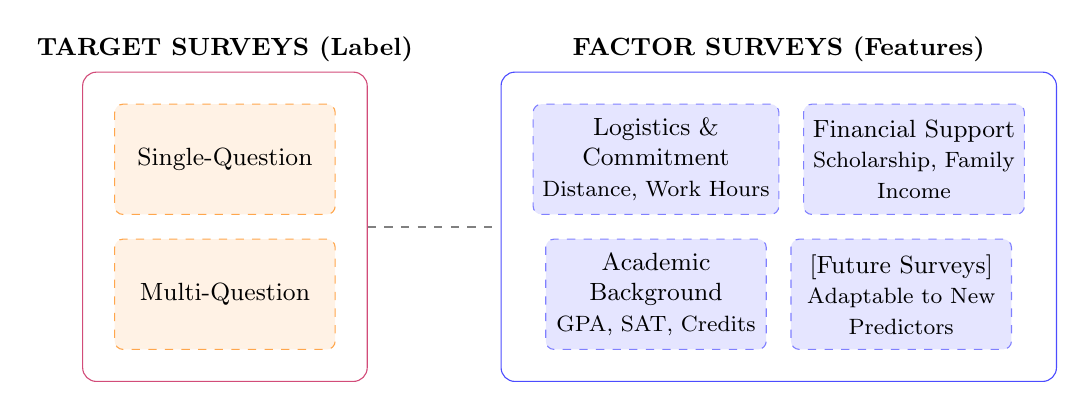
\begin{tikzpicture}[
  box/.style={draw,dashed,rounded corners=3pt,minimum width=28mm,minimum height=14mm,align=center,font=\small},
  target/.style={box,draw=orange!70,fill=orange!10},
  factor/.style={box,draw=blue!50,fill=blue!10},
  container/.style={draw,rounded corners=5pt,inner sep=4mm}
]
% Target surveys
\node[target] (sq) {Single-Question};
\node[target,below=3mm of sq] (mq) {Multi-Question};
\node[container,draw=purple!70,fit=(sq)(mq),label={[font=\small\bfseries]above:TARGET SURVEYS (Label)}] (tbox) {};

% Factor surveys
\node[factor,right=25mm of sq] (lc) {Logistics \&\\Commitment\\{\footnotesize Distance, Work Hours}};
\node[factor,right=3mm of lc] (fs) {Financial Support\\{\footnotesize Scholarship, Family}\\{\footnotesize Income}};
\node[factor,below=3mm of lc] (ab) {Academic\\Background\\{\footnotesize GPA, SAT, Credits}};
\node[factor,right=3mm of ab] (fu) {[Future Surveys]\\{\footnotesize Adaptable to New}\\{\footnotesize Predictors}};
\node[container,draw=blue!70,fit=(lc)(fs)(ab)(fu),label={[font=\small\bfseries]above:FACTOR SURVEYS (Features)}] (fbox) {};

% Connection
\draw[gray,dashed,thick] (tbox.east) -- (fbox.west);
\end{tikzpicture}
}%
\caption{Dual-Survey Architecture. Target Surveys collect the outcome ($Y$), Factor Surveys collect predictors ($X$). Dashed lines show linkage relationships enabling flexible study configurations.}
\label{fig:dualsurvey}
\end{figure}

\subsection{Architectural Philosophy: Small Data by Design}\label{subsec:progressive}

ACOSUS addresses data scarcity constraints through a framework that treats them not as limitations to overcome but as fundamental design constraints to embrace. The architecture ensures the system delivers value from the very first student enrollment—before any predictions are possible, advisors gain access to structured student profiles through standardized data collection instruments. This immediate utility transforms the cold-start period from a limitation into a productive data-gathering phase.

\subsubsection{The Three-Stage Progressive Pipeline}

As observations accumulate, the system's predictive intelligence matures through a three-stage progressive pipeline:

\textbf{Foundation Stage.} The system prioritizes collecting high-quality labeled observations through survey instruments that capture both outcomes and predictive features. Once a minimal corpus exists, lightweight predictive methods generate initial predictions---this stage emphasizes data quality over prediction sophistication, establishing a reliable foundation for subsequent phases.

\textbf{Augmentation Stage.} As the corpus grows, this stage addresses the fundamental small-sample limitation through generative techniques that synthesize additional training observations. These methods learn distributional characteristics from authentic data and produce synthetic samples that expand the training corpus while preserving statistical properties, providing sufficient volume to support more sophisticated algorithms.

\textbf{Refinement Stage.} Finally, the system transitions to advanced non-linear models capable of capturing complex feature-outcome relationships. 

The framework's modularity extends beyond the three-stage progression. Each computational component operates as an interchangeable module: any predictive method may serve the foundation stage, any generative technique may perform augmentation, and any deep learning architecture may handle refinement. This algorithm-agnostic design serves two purposes in the small-data context. First, it enables empirical comparison---researchers can evaluate which specific algorithms perform best with limited transfer student observations rather than committing to a fixed approach. Second, as methodological advances emerge in few-shot learning, data augmentation, or neural architecture design, the framework can integrate these improvements without structural modification---positioning ACOSUS not as a fixed implementation but as a generalizable architecture adaptable to diverse educational prediction contexts.

% Figure 4 - Three-Stage Progressive Pipeline diagram
\begin{figure}[htbp]
\centering
\resizebox{\textwidth}{!}{%
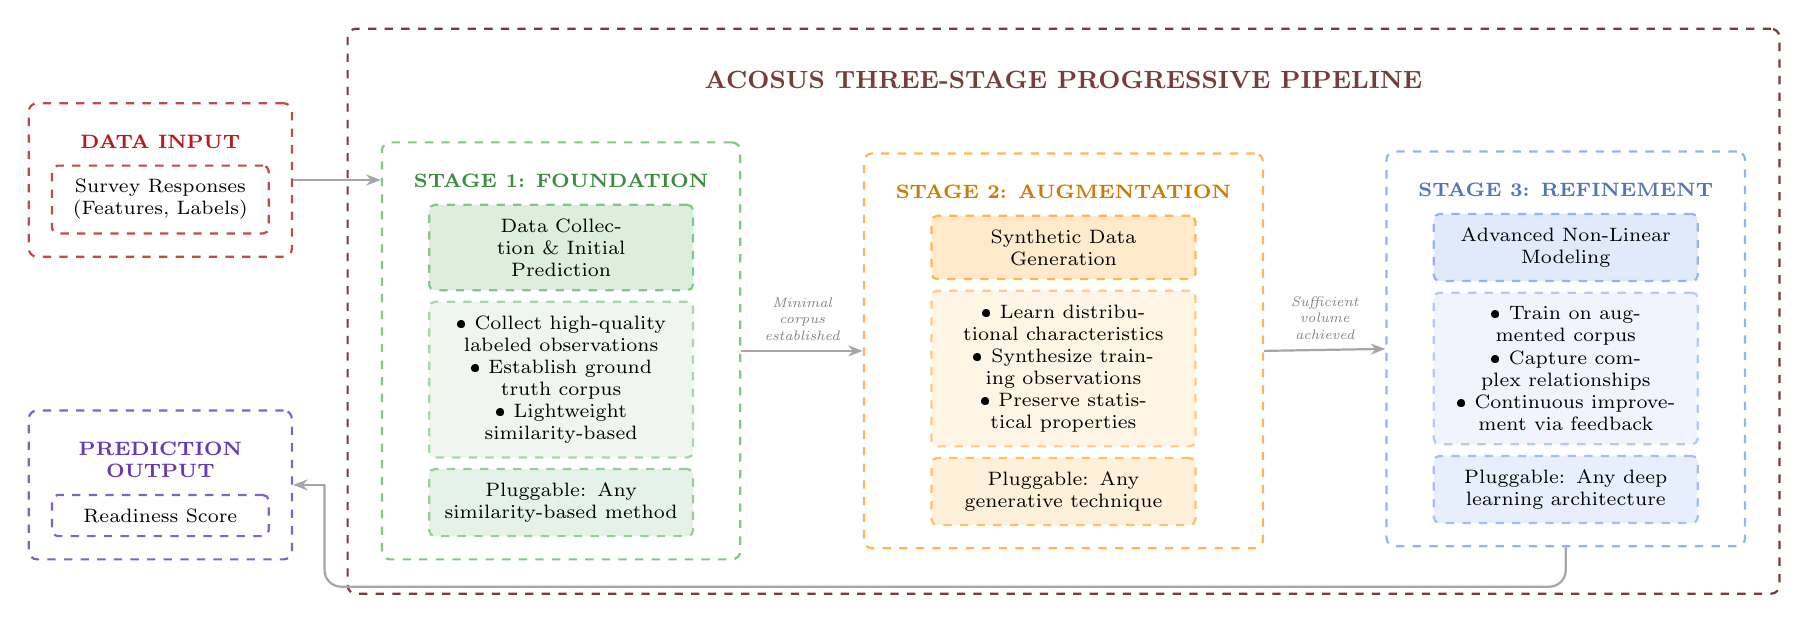
\begin{tikzpicture}[
    node distance=0.3cm,
    inner/.style={rectangle, dashed, thick, rounded corners=2pt, align=center, inner sep=5pt, font=\scriptsize},
    outer/.style={rectangle, dashed, thick, rounded corners=3pt, inner sep=8pt},
    header/.style={inner, fill=#1!20, draw=#1!70},
    content/.style={inner, fill=#1!10, draw=#1!50},
    plug/.style={inner, fill=#1!15, draw=#1!60},
    arrow/.style={-{Stealth[scale=0.8]}, gray!70, thick},
    lbl/.style={font=\tiny\itshape, text=gray, align=center}
]

% Stage 1 inner boxes
\node[header=stage1, text width=3cm] (s1-head) {Data Collection \& Initial\\Prediction};
\node[content=stage1, below=0.12cm of s1-head, text width=3cm] (s1-content) {
    \textbullet\ Collect high-quality labeled observations\\
    \textbullet\ Establish ground truth corpus\\
    \textbullet\ Lightweight similarity-based
};
\node[plug=stage1, below=0.12cm of s1-content, text width=3cm] (s1-plug) {Pluggable: Any\\similarity-based method};
\node[above=0.08cm of s1-head, font=\scriptsize\bfseries, text=stage1!80!black] (s1-title) {STAGE 1: FOUNDATION};
\node[outer, draw=stage1!70, fit=(s1-title)(s1-head)(s1-content)(s1-plug)] (stage1-box) {};

% Stage 2 inner boxes
\node[header=stage2, right=3cm of s1-head, text width=3cm] (s2-head) {Synthetic Data\\Generation};
\node[content=stage2, below=0.12cm of s2-head, text width=3cm] (s2-content) {
    \textbullet\ Learn distributional characteristics\\
    \textbullet\ Synthesize training observations\\
    \textbullet\ Preserve statistical properties
};
\node[plug=stage2, below=0.12cm of s2-content, text width=3cm] (s2-plug) {Pluggable: Any\\generative technique};
\node[above=0.08cm of s2-head, font=\scriptsize\bfseries, text=stage2!80!black] (s2-title) {STAGE 2: AUGMENTATION};
\node[outer, draw=stage2!70, fit=(s2-title)(s2-head)(s2-content)(s2-plug)] (stage2-box) {};

% Stage 3 inner boxes
\node[header=stage3, right=3cm of s2-head, text width=3cm] (s3-head) {Advanced Non-Linear\\Modeling};
\node[content=stage3, below=0.12cm of s3-head, text width=3cm] (s3-content) {
    \textbullet\ Train on augmented corpus\\
    \textbullet\ Capture complex relationships\\
    \textbullet\ Continuous improvement via feedback
};
\node[plug=stage3, below=0.12cm of s3-content, text width=3cm] (s3-plug) {Pluggable: Any deep\\learning architecture};
\node[above=0.08cm of s3-head, font=\scriptsize\bfseries, text=stage3!80!black] (s3-title) {STAGE 3: REFINEMENT};
\node[outer, draw=stage3!70, fit=(s3-title)(s3-head)(s3-content)(s3-plug)] (stage3-box) {};

% Pipeline title (centered above stages)
\path (stage1-box.north west) -- (stage3-box.north east) coordinate[midway] (pipeline-center);
\node[above=0.6cm of pipeline-center, font=\small\bfseries, text=pipelineborder] (pipeline-title) {ACOSUS THREE-STAGE PROGRESSIVE PIPELINE};

% Pipeline outer box
\begin{scope}[on background layer]
\node[outer, draw=pipelineborder, fit=(pipeline-title)(stage1-box)(stage2-box)(stage3-box), inner sep=12pt] (pipeline) {};
\end{scope}

% Input box (aligned to top of pipeline)
\node[inner, fill=white, draw=inputred!80, text width=2.4cm, anchor=north] at ([xshift=-2.8cm]stage1-box.north west |- s1-title.north) (input-inner) {Survey Responses\\(Features, Labels)};
\node[above=0.08cm of input-inner, font=\scriptsize\bfseries, text=inputred] (input-title) {DATA INPUT};
\node[outer, draw=inputred!80, fit=(input-title)(input-inner)] (input-box) {};

% Output box (aligned to bottom of pipeline, same size as input)
\node[inner, fill=white, draw=outputviolet!80, text width=2.4cm, anchor=south] at ([xshift=-2.8cm]stage1-box.south west |- s1-plug.south) (output-inner) {Readiness Score};
\node[above=0.08cm of output-inner, font=\scriptsize\bfseries, text=outputviolet, align=center] (output-title) {PREDICTION\\ OUTPUT};
\node[outer, draw=outputviolet!80, fit=(output-title)(output-inner)] (output-box) {};

% Arrows
\draw[arrow] (input-box.east) -- (stage1-box.west |- input-box.east);
\draw[arrow] (stage1-box.east) -- node[lbl, above] {Minimal\\corpus\\established} (stage2-box.west);
\draw[arrow] (stage2-box.east) -- node[lbl, above] {Sufficient\\volume\\achieved} (stage3-box.west);

% Feedback arrow
\coordinate (turn1) at ([yshift=-0.5cm]stage3-box.south);
\coordinate (turn2) at (turn1 -| output-box.east);
\coordinate (turn3) at ([xshift=0.4cm]output-box.east);
\draw[gray!70, thick, rounded corners=6pt] (stage3-box.south) -- (turn1) -- (turn1 -| turn3) -- (turn3);
\draw[arrow] (turn3) -- (output-box.east);

\end{tikzpicture}
}%
\caption{The Three-Stage Progressive Pipeline. Each stage represents a pluggable component that can be substituted with alternative algorithms. The framework progresses from data acquisition through augmentation to refined prediction, with feedback loops enabling continuous improvement.}
\label{fig:pipeline}
\end{figure}

%%%%%%%%%%%%%%%%%%%%%%%%%%%%%%%%%%%%%%%%%%%%%%%%%
% SECTION 4: SYSTEM IMPLEMENTATION
%%%%%%%%%%%%%%%%%%%%%%%%%%%%%%%%%%%%%%%%%%%%%%%%%
\section{System Implementation}\label{sec:implementation}

The ACOSUS platform translates the architectural principles described in Section~\ref{sec:design} into a functional system. This section details how survey instruments capture and process heterogeneous student data (\S\ref{subsec:dataprocessing}), the layered system architecture that supports both prediction and advising workflows (\S\ref{subsec:sysarch}), and the configuration flexibility that enables researchers to adapt the framework to diverse institutional contexts (\S\ref{subsec:config}).

\subsection{Survey Data Processing}\label{subsec:dataprocessing}

The survey instruments described in Section~\ref{subsec:dualsurvey} synthesize information collected from students into feature vectors suitable for predictive modeling. Each survey question serves as a proxy for an underlying success factor identified in prior research---our factor analysis work established mappings between observable indicators (e.g., scholarship status, commute distance) and latent constructs (e.g., financial stability, institutional commitment) that predict transfer student outcomes \cite{factoranalysis2023}.

\subsubsection{Priority Weighting}

Not all factors contribute equally to student success. Research on transfer student outcomes consistently identifies certain variables---academic self-efficacy, financial stability, institutional fit---as more predictive than others \cite{factoranalysis2023,computingtransfer2024,socialcognitive2022}. ACOSUS operationalizes this differential importance through \textbf{priority scores}: These priorities derive from empirical evidence (effect sizes and factor loadings from prior research) and can be dynamically adjusted as advisor feedback identifies which factors prove most predictive for specific institutional contexts.

The priority-weighted aggregation follows a straightforward formulation. For a survey with $n$ questions, where question $i$ has priority score $p_i$, the student selects an option with weightage $w_i^{\text{selected}}$ from a maximum possible $w_i^{\text{max}}$:

\begin{equation}
S = \frac{\sum_{i=1}^{n} \left(\frac{w_i^{\text{selected}}}{w_i^{\text{max}}} \times p_i\right)}{\sum_{i=1}^{n} p_i}
\label{eq:priority}
\end{equation}

This yields a normalized score in $[0, 1]$ that accounts for both response quality and question importance. A logistic calibration curve is then applied to prevent overconfident predictions at the extremes.

\begin{table}[htbp]
\centering
\caption{Example priority score assignments based on literature-informed importance.}
\label{tab:priority}
\begin{tabular}{@{}p{3.2cm}p{4.5cm}cp{3.5cm}@{}}
\toprule
\textbf{Factor Category} & \textbf{Example Question} & \textbf{Priority} & \textbf{Rationale} \\
\midrule
Academic Self-Efficacy & How confident in your ability to succeed? & 9 & Strong predictor \cite{bandura1997} \\
\midrule
Financial Stability & Expected financial stress impact? & 8 & Affects retention \cite{socialcognitive2022} \\
\midrule
Institutional Commitment & How committed to completing this program? & 9 & Persistence indicator \cite{tinto1993} \\
\midrule
Logistics & Commute distance to university? & 6 & Practical barrier \\
\bottomrule
\end{tabular}
\end{table}

This priority-weighted approach offers an additional advantage: the weights can serve as informative priors in probabilistic modeling frameworks. When the system transitions to more sophisticated prediction methods, priority scores provide a principled initialization---features with higher priorities receive greater initial influence, which the model can then refine based on observed data. This connection between expert knowledge and learned parameters supports Bayesian inference approaches where priority weights inform prior distributions over feature importance.

\subsubsection{Data Type Handling}

Survey responses encompass heterogeneous data types that require type-aware normalization before model ingestion. The distinction between \textbf{ordinal} and \textbf{cardinal} data is particularly important: ordinal responses (e.g., ``Not confident'' $<$ ``Somewhat confident'' $<$ ``Very confident'') carry inherent ordering that must be preserved, while cardinal responses (e.g., career aspiration categories) represent nominal distinctions without implied ranking.

\begin{table}[htbp]
\centering
\caption{Normalization strategies for different data types.}
\label{tab:normalization}
\begin{tabular}{@{}lll@{}}
\toprule
\textbf{Data Type} & \textbf{Example} & \textbf{Normalization Method} \\
\midrule
Ordinal & GPA range: ``3.0--3.5'' & Direct option weightage (e.g., 8/10) \\
Cardinal & Career: ``Industry/Corporate'' & Equal weightage or domain-specific mapping \\
Continuous & SAT score: 1250 & Min-max scaling: $(x - \min)/(\max - \min)$ \\
\bottomrule
\end{tabular}
\end{table}

This type-aware processing ensures that the semantic meaning of responses is preserved during feature engineering---ordinal relationships remain ordered, nominal categories are not spuriously ranked, and continuous values are appropriately scaled.

% Figure 5 - Survey Data Processing Pipeline diagram
\begin{figure}[htbp]
\centering
\resizebox{0.95\textwidth}{!}{%
\begin{tikzpicture}[
    node distance=0.35cm,
    inner/.style={rectangle, dashed, thick, rounded corners=3pt, align=center, inner sep=10pt, font=\normalsize},
    outer/.style={rectangle, thick, rounded corners=3pt, inner sep=6pt},
    arrow/.style={-{Stealth[scale=0.9]}, gray!70, thick, rounded corners=6pt},
    arrowline/.style={gray!70, thick, rounded corners=6pt}
]

% Survey Collection inner boxes
\node[inner, fill=surveyboxfill, draw=surveyblue!70, text width=3cm, minimum height=0.75cm] (q1) {Question 1\\(Ordinal)};
\node[inner, fill=surveyboxfill, draw=surveyblue!70, text width=3cm, minimum height=.75cm, below=0.2cm of q1] (q2) {Question 2\\(Cardinal)};
\node[inner, fill=surveyboxfill!40, draw=surveyblue!40, densely dotted, text width=3cm, minimum height=.75cm, below=0.2cm of q2] (qdots) {\textit{...}};
\node[inner, fill=surveyboxfill, draw=surveyblue!70, text width=3cm, minimum height=0.75cm, below=0.2cm of qdots] (qn) {Question N\\(Continuous)};

% Survey Collection title and outer box
\node[above=0.3cm of q1, font=\normalsize\bfseries, text=surveyblue!80!black] (survey-title) {SURVEY COLLECTION};
\node[outer, draw=surveyblue, fit=(survey-title)(q1)(q2)(qdots)(qn), inner sep=10pt] (survey-box) {};

% Data Processing inner boxes
\node[inner, fill=processboxfill, draw=processboxborder, text width=3cm, minimum height=1cm, right=1.8cm of q1.east |- q1.south east] (priority) {Priority\\Weighting};
\node[inner, fill=processboxfill, draw=processboxborder, text width=3cm, minimum height=1cm, below=0.8cm of priority] (normalize) {Type-Aware\\Normalization};

% Data Processing title and outer box
\node[above=0.3cm of priority, font=\normalsize\bfseries, text=processorange!80!black] (process-title) {DATA PROCESSING};
\node[outer, draw=processorange, fit=(process-title)(priority)(normalize), inner sep=10pt] (process-box) {};

% Model Input inner box (centered with process box)
\path (priority.center) -- (normalize.center) coordinate[midway] (process-center);
\node[inner, fill=modelboxfill, draw=modelboxborder, text width=3cm, minimum height=1cm, right=1.5cm of process-box.east, anchor=west] (feature) {Normalized\\Feature Vector};

% Model Input title and outer box
\node[above=0.3cm of feature, font=\normalsize\bfseries, text=modelgreen] (model-title) {MODEL INPUT};
\node[outer, draw=modelgreen, fit=(model-title)(feature), inner sep=10pt] (model-box) {};

% Arrows from Survey to Priority Weighting (converging)
% Merge point at Q2 level so Q2 has straight horizontal line
\coordinate (merge-point) at ($(survey-box.east)!0.5!(process-box.west) |- q2$);

% Curved lines from questions converging to merge point, then to priority
\draw[arrowline] (q1.east) to[out=0, in=135] (merge-point);
\draw[arrowline] (q2.east) -- (merge-point);
\draw[arrowline] (qn.east) to[out=0, in=-135] (merge-point);
\draw[arrow] (merge-point) to[out=45, in=180] (priority.west);

% Arrow between Priority and Normalization
\draw[arrow] (priority.south) -- (normalize.north);

% Arrow from Normalization to Feature Vector
\draw[arrowline] (normalize.east) -- (process-box.east |- normalize.east);
\draw[arrow] (process-box.east |- normalize.east) to[out=0, in=180] (feature.west);

\end{tikzpicture}
}%
\caption{Survey data processing pipeline. Raw responses undergo priority weighting and type-aware normalization to produce standardized feature vectors for model ingestion.}
\label{fig:processing}
\end{figure}

\subsection{System Architecture}\label{subsec:sysarch}

The ACOSUS platform implements a four-layer architecture that separates concerns across presentation, business logic, data persistence, and predictive modeling (Figure~\ref{fig:architecture}). This separation enables independent scaling of each layer and supports the system's dual purpose: serving student-facing predictions while centralizing advisor-facing information.

The \textbf{Presentation Layer} provides role-specific interfaces through a web-based application. Students access survey completion workflows, view predictions, and submit feedback. Advisors access a unified dashboard that consolidates student profiles---organized by the same categories as Factor Surveys---eliminating the need to gather information from disparate sources. Administrators configure survey instruments, trigger model training, and monitor system analytics.

The \textbf{Business Logic Layer} orchestrates application workflows, enforcing the progressive learning framework's phase transitions. This layer ensures students encounter appropriate interfaces based on current system state---data collection only during the foundation phase, prediction with feedback during subsequent phases.

The \textbf{Data Layer} provides flexible document storage for users, surveys, responses, and model metadata. The schema-flexible design accommodates researcher-defined survey instruments without requiring database migrations as questions evolve.

The \textbf{Model Layer} operates as a separate service handling computationally intensive tasks: data normalization, prediction inference across all three pipeline stages, and model training. Asynchronous job queues prevent long-running training tasks from blocking prediction requests. Model versioning ensures that only validated improvements reach production---new models must demonstrate improved accuracy on held-out real student data before deployment.

% Figure 6 - System Architecture diagram
\begin{figure}[htbp]
\centering
\resizebox{0.95\textwidth}{!}{%
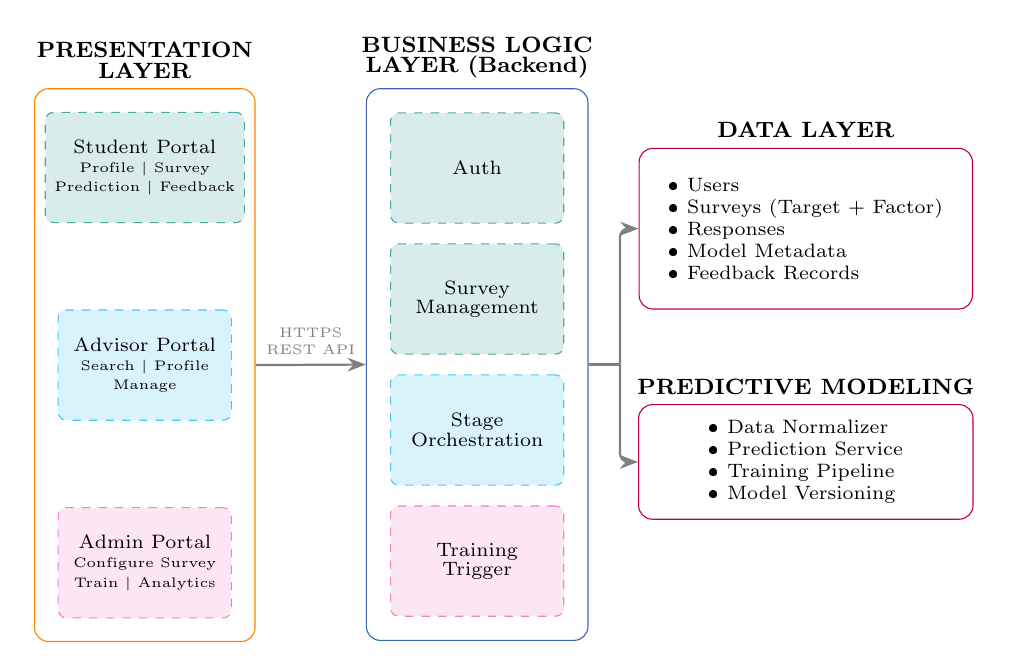
\begin{tikzpicture}[
    node distance=2.5mm,
    box/.style={draw, dashed, rounded corners=3pt, minimum width=22mm, minimum height=14mm, align=center, font=\scriptsize},
    layer/.style={draw, rounded corners=5pt, inner sep=3mm},
    student/.style={box, draw=teal!70, fill=teal!15},
    advisor/.style={box, draw=cyan!70, fill=cyan!15},
    admin/.style={box, draw=magenta!50, fill=magenta!10},
    lbl/.style={font=\footnotesize\bfseries, align=center},
    >=Stealth
]

% Column 2: Business Logic Layer (reference)
\node[student] (auth) {Auth};
\node[student, below=of auth] (surv) {Survey\\[-1pt]Management};
\node[advisor, below=of surv] (stage) {Stage\\[-1pt]Orchestration};
\node[admin, below=of stage] (train) {Training\\[-1pt]Trigger};

\begin{scope}[on background layer]
\node[layer, draw=dblue, fit=(auth)(surv)(stage)(train), label={[lbl]above:BUSINESS LOGIC\\[-2pt]LAYER (Backend)}] (biz) {};
\end{scope}

% Column 1: Presentation Layer - create outer box first, then place inner boxes
\path let \p1=(biz.north), \p2=(biz.south), \p3=(biz.west) in
    node[layer, draw=orange,
         minimum height={\y1-\y2},
         minimum width=28mm,
         anchor=north east,
         label={[lbl]above:PRESENTATION\\[-2pt]LAYER}] (pres) at ($(\x3,\y1)+(-14mm,0)$) {};

% Place boxes centered inside pres
\node[student, anchor=north] at ($(pres.north)+(0,-3mm)$) (sp) {Student Portal\\[-1pt]\tiny Profile \textbar{} Survey\\[-1pt]\tiny Prediction \textbar{} Feedback};
\node[advisor] at (pres.center) (ap) {Advisor Portal\\[-1pt]\tiny Search \textbar{} Profile\\[-1pt]\tiny Manage};
\node[admin, anchor=south] at ($(pres.south)+(0,3mm)$) (adm) {Admin Portal\\[-1pt]\tiny Configure Survey\\[-1pt]\tiny Train \textbar{} Analytics};

% Column 3: Data Layer (top) + ML Layer (bottom)
\node[right=12mm of auth, font=\scriptsize, align=left, anchor=north west] (dlist) {
    \textbullet\ Users\\
    \textbullet\ Surveys (Target + Factor)\\
    \textbullet\ Responses\\
    \textbullet\ Model Metadata\\
    \textbullet\ Feedback Records
};

\begin{scope}[on background layer]
\node[layer, draw=purple, fit=(dlist), inner sep=2.5mm, label={[lbl]above:DATA LAYER}] (data) {};
\end{scope}

% Predictive Modeling Layer - match Data Layer size
\path let \p1=(data.north), \p2=(data.south), \p3=(data.west), \p4=(data.east) in
    node[below=12mm of data, layer, draw=purple, minimum height={\y1-\y2-6mm}, minimum width={\x4-\x3}, label={[lbl]above:PREDICTIVE MODELING}] (ml) {};

\node[font=\scriptsize, align=left] at (ml.center) {
    \textbullet\ Data Normalizer\\
    \textbullet\ Prediction Service\\
    \textbullet\ Training Pipeline\\
    \textbullet\ Model Versioning
};

% Title
%\node[font=\large\bfseries, above=12mm of biz.north] (title) {ACOSUS SYSTEM ARCHITECTURE};

% Arrows
\draw[->, thick, gray] (pres.east) -- (biz.west) node[midway, above, font=\tiny, align=center] {HTTPS\\REST API};
\coordinate (split) at ($(biz.east)+(4mm,0)$);
\draw[thick, gray] (biz.east) -- (split);
\draw[->, thick, gray, rounded corners=3pt] (split) |- (data.west);
\draw[->, thick, gray, rounded corners=3pt] (split) |- (ml.west);

\end{tikzpicture}
}%
\caption{ACOSUS system architecture. Four layers separate presentation, business logic, data persistence, and predictive modeling, enabling independent scaling and clear separation of responsibilities.}
\label{fig:architecture}
\end{figure}

\subsection{Model Configuration Flexibility}\label{subsec:config}

The algorithm-agnostic design described in Section~\ref{subsec:progressive} manifests in a configuration system that allows researchers to adapt the framework without modifying core infrastructure. Four categories of configuration support this flexibility:

\textbf{Survey Linkage:} The dual-survey architecture described in Section~\ref{subsec:dualsurvey} is operationalized through explicit linkage configurations. A single Target Survey (outcome $Y$) may be linked to multiple Factor Surveys (predictor sets $X_1, X_2, X_3$), enabling researchers to investigate which predictor combinations best predict success. This linkage mechanism provides several research advantages:

\begin{enumerate}
    \item \textbf{Comparative predictor analysis}---researchers can deploy alternative Factor Surveys to the same cohort and compare predictive validity across different predictor sets;
    \item \textbf{Longitudinal adaptability}---as research identifies new predictors of transfer success (e.g., post-pandemic factors, emerging transfer shock indicators), new Factor Surveys can be added without disrupting existing data collection or invalidating historical comparisons;
    \item \textbf{Cohort customization}---different academic programs can deploy program-specific Factor Surveys (e.g., technical preparation for computing majors) while maintaining a common outcome measure through shared Target Surveys.
\end{enumerate}

% Figure 7 - Dual-Survey Architecture with Linkage
\begin{figure}[htbp]
\centering
\resizebox{0.95\textwidth}{!}{%
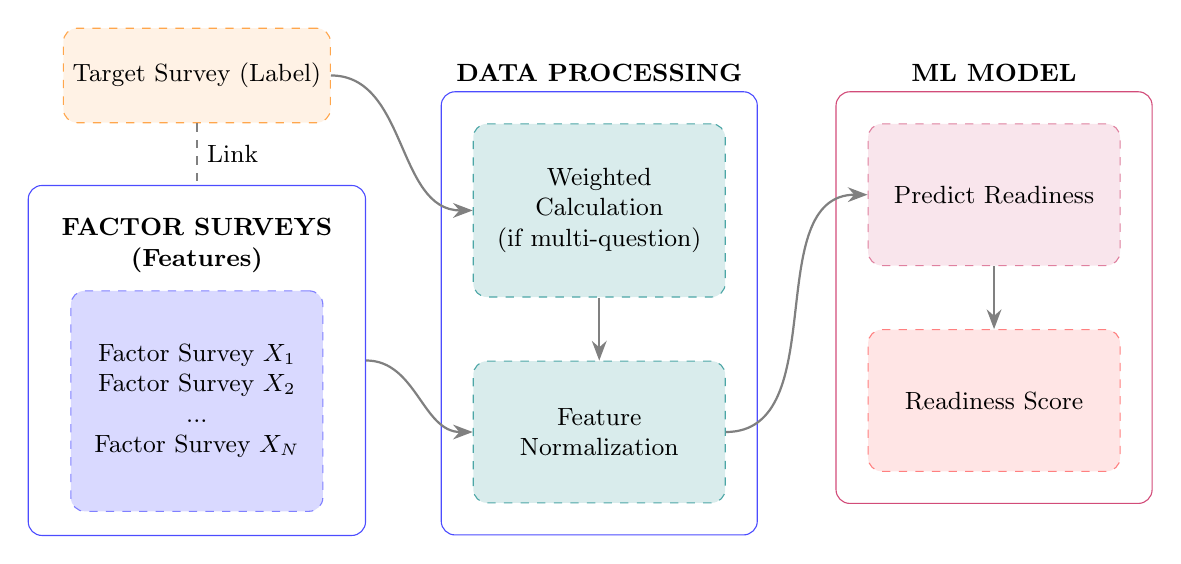
\begin{tikzpicture}[
  box/.style={draw,dashed,rounded corners=5pt,align=center,font=\small},
  container/.style={draw,rounded corners=5pt,inner sep=4mm},
  arr/.style={gray,thick,-{Stealth[length=2.5mm]}}
]
% Left column - Target Survey
\node[box,draw=orange!70,fill=orange!10,minimum width=32mm,minimum height=12mm] (target) {Target Survey (Label)};

% Middle column - Data Processing
\node[box,draw=teal!70,fill=teal!15,minimum width=32mm,minimum height=22mm,right=18mm of target.south east,anchor=north west] (weighted) {Weighted\\Calculation\\(if multi-question)};
\node[box,draw=teal!70,fill=teal!15,minimum width=32mm,minimum height=18mm,below=8mm of weighted] (normalize) {Feature\\Normalization};
\node[container,draw=blue!70,fit=(weighted)(normalize),label={[font=\small\bfseries]above:DATA PROCESSING}] (dbox) {};

% Left column - Factor Surveys (aligned to dbox bottom)
\node[box,draw=blue!50,fill=blue!15,minimum width=32mm,minimum height=28mm,anchor=south] at ([yshift=3mm]target.south|-dbox.south) (factors) {Factor Survey $X_1$\\Factor Survey $X_2$\\...\\Factor Survey $X_N$};
\node[font=\small\bfseries,align=center,above=1mm of factors] (flabel) {FACTOR SURVEYS\\(Features)};
\node[container,draw=blue!70,inner sep=3mm,fit=(factors)(flabel)] (fbox) {};

% Link between target and factor surveys
\draw[gray,dashed,thick] (target.south) -- node[right,font=\small,black]{Link} (fbox.north);

% Right column - ML Model
\node[box,draw=purple!50,fill=purple!10,minimum width=32mm,minimum height=18mm,right=18mm of weighted.north east,anchor=north west] (predict) {Predict Readiness};
\node[box,draw=red!50,fill=red!10,minimum width=32mm,minimum height=18mm,below=8mm of predict] (score) {Readiness Score};
\node[container,draw=purple!70,fit=(predict)(score),label={[font=\small\bfseries]above:ML MODEL}] (mbox) {};

% Arrows
\draw[arr] (target.east) to[out=0,in=180] (weighted.west);
\draw[arr] (fbox.east) to[out=0,in=180] (normalize.west);
\draw[arr] (weighted.south) -- (normalize.north);
\draw[arr] (normalize.east) to[out=0,in=180] (predict.west);
\draw[arr] (predict.south) -- (score.north);
\end{tikzpicture}
}%
\caption{Dual-Survey Architecture with survey linkage. Dashed lines show linkage relationships between Target and Factor Surveys, enabling flexible study configurations where a single outcome measure can be associated with multiple predictor sets.}
\label{fig:linkage}
\end{figure}

The remaining three categories address the progressive learning pipeline:

\textbf{Phase Transition Thresholds.} Administrators specify the observation counts that trigger transitions between pipeline stages. Default thresholds reflect statistical considerations for each algorithm family, but institutions can adjust these boundaries based on their enrollment patterns and desired trade-offs between prediction availability and model reliability.

\textbf{Algorithm Selection:} Each pipeline stage accepts any algorithm conforming to the expected interface. The \textbf{foundation stage} requires a predictor that operates effectively with minimal training data---any similarity-based or instance-based method satisfies this constraint. The \textbf{augmentation stage} requires a generative model capable of synthesizing observations that preserve distributional properties. The \textbf{refinement stage} accepts any supervised learning architecture capable of capturing non-linear relationships. This modularity enables empirical comparison: researchers can evaluate alternative algorithms on their specific student population rather than accepting default choices.

\textbf{Hyperparameter Tuning:} Within each algorithm, configurable parameters allow fine-tuning for institutional context. Distance metrics, neighbor counts, generation multipliers, network architectures, and training schedules are all exposed as configuration options. The system logs all configuration choices alongside model performance metrics, enabling systematic comparison across settings.

This configuration flexibility supports the framework's positioning as a generalizable architecture rather than a fixed implementation. As methodological advances emerge---improved few-shot learning techniques, more effective data augmentation strategies, novel neural architectures---institutions can integrate these improvements by updating configuration rather than reengineering the system.

%%%%%%%%%%%%%%%%%%%%%%%%%%%%%%%%%%%%%%%%%%%%%%%%%
% SECTION 5: EVALUATION
%%%%%%%%%%%%%%%%%%%%%%%%%%%%%%%%%%%%%%%%%%%%%%%%%
\section{Evaluation}\label{sec:evaluation}

To assess the usability and perceived value of the ACOSUS platform, we conducted a pilot study with transfer students at a public urban university. This section describes the study design (\S\ref{subsec:studydesign}), evaluation instruments (\S\ref{subsec:instruments}), quantitative results (\S\ref{subsec:quantresults}), and qualitative findings (\S\ref{subsec:qualfindings}).

\subsection{Study Design}\label{subsec:studydesign}

\subsubsection{Participants}

Four transfer students ($N=4$) from Northeastern Illinois University participated in the study. Participants were recruited through email invitation and voluntarily enrolled after providing informed consent. All participants were active transfer students in computing-related majors. This evaluation was conducted during the foundation phase of the progressive learning pipeline (Section~\ref{subsec:progressive}), when the system was actively collecting labeled observations to establish the initial training corpus. At this stage, no predictive model had yet been trained---the system's primary function was structured data collection rather than prediction generation. Participants completed the Factor and Target Survey instruments described in Sections~\ref{subsec:dualsurvey} and~\ref{subsec:dataprocessing}, followed by a post-hoc feedback survey administered through Qualtrics. The study protocol received the University's Institutional Review Board (IRB) approval prior to data collection.

\subsection{Evaluation Instruments}\label{subsec:instruments}

The feedback survey was designed based on the Technology Acceptance Model (TAM) framework \cite{davis1989} to assess participants' perceptions of the data collection experience. The instruments are mainly comprised of Likert-scale items (5-point scale) measuring Perceived Usefulness, Perceived Ease of Use, and Behavioral Intention, along with open-ended questions capturing qualitative feedback on interface difficulties, helpful features, missing capabilities, and redesign suggestions. Table~\ref{tab:constructs} presents the constructs and example items.

\begin{table}[htbp]
\centering
\caption{Feedback survey constructs and items.}
\label{tab:constructs}
\begin{tabular}{@{}lp{8cm}@{}}
\toprule
\textbf{Construct} & \textbf{Example Item} \\
\midrule
Perceived Usefulness (PU) & ``Using this AI counseling system enables me to accomplish tasks more quickly than other advising methods.'' \\
Perceived Ease of Use (PEOU) & ``Learning to operate this AI counseling system was easy for me.'' \\
Behavioral Intention & ``How likely are you to continue using this system for academic planning?'' \\
\bottomrule
\end{tabular}
\end{table}

Open-ended questions captured qualitative feedback on interface difficulties, helpful features, missing capabilities, and redesign suggestions.

\subsection{Quantitative Results}\label{subsec:quantresults}

\subsubsection{TAM Construct Scores}

Analysis of the TAM-based constructs revealed strong positive perceptions across all dimensions.

\begin{table}[htbp]
\centering
\caption{Summary statistics for evaluation metrics (5-point Likert scale).}
\label{tab:results}
\begin{tabular}{@{}lcccc@{}}
\toprule
\textbf{Metric} & \textbf{Mean} & \textbf{SD} & \textbf{Min} & \textbf{Max} \\
\midrule
Perceived Usefulness (PU) & 4.46 & 0.85 & 3 & 5 \\
Perceived Ease of Use (PEOU) & 5.00 & 0.00 & 5 & 5 \\
Likelihood to Continue & 4.75 & 0.50 & 4 & 5 \\
Likelihood to Recommend & 4.25 & 1.50 & 2 & 5 \\
\bottomrule
\end{tabular}
\end{table}

% Figure 7 - TAM construct scores
\begin{figure}[htbp]
\centering
\includegraphics[width=0.9\textwidth]{infographics/fig1_tam_metrics.png}
\caption{TAM construct scores. Perceived Ease of Use achieved a perfect score ($M=5.00$), while Perceived Usefulness showed strong agreement ($M=4.46$) with slightly more variance.}
\label{fig:tam}
\end{figure}

Perceived Ease of Use achieved a perfect mean score ($M=5.00$, $SD=0.00$), indicating that all participants found the system straightforward to learn and operate. Perceived Usefulness was rated highly ($M=4.46$, $SD=0.85$), though with greater variance reflecting individual differences in how participants valued the system's utility for their specific situations.

\subsubsection{Behavioral Intention}

% Figure 10 - Behavioral intention metrics
\begin{figure}[htbp]
\centering
\includegraphics[width=0.9\textwidth]{infographics/fig4_behavioral_intention.png}
\caption{Behavioral intention. Likelihood to Continue ($M=4.75$) exceeded Likelihood to Recommend ($M=4.25$), with the latter showing greater variance.}
\label{fig:behavioral}
\end{figure}

Likelihood to Continue using the system was high ($M=4.75$, $SD=0.50$), suggesting strong personal adoption intent. Likelihood to Recommend showed more variance ($M=4.25$, $SD=1.50$), with one participant providing a lower rating (2/5). This discrepancy may reflect individual differences in social recommendation behavior rather than system satisfaction.

\subsection{Qualitative Findings}\label{subsec:qualfindings}

Thematic analysis of open-ended responses revealed four primary themes.

% Figure 16 - Qualitative theme distribution
\begin{figure}[htbp]
\centering
\includegraphics[width=0.9\textwidth]{infographics/fig6_qualitative_themes.png}
\caption{Qualitative theme distribution. UI/Navigation Positive was the most frequently occurring theme (4 mentions), followed by No Issues Reported (3), Personalization Request (2), and Speed/Efficiency (1).}
\label{fig:themes}
\end{figure}

\begin{table}[htbp]
\centering
\caption{Qualitative themes and representative responses.}
\label{tab:themes}
\begin{tabular}{@{}lcp{7cm}@{}}
\toprule
\textbf{Theme} & \textbf{Count} & \textbf{Representative Quote} \\
\midrule
Usability & 3 & ``UI navigation is very user friendly''; ``User interface was easy to understand and navigate'' \\
Satisfaction & 3 & ``No feature was missing, experience was great''; ``None, everything was clear'' \\
Efficiency & 1 & ``Faster and more compatible'' \\
Personalization & 1 & ``Make it tailored more towards individual users'' \\
\bottomrule
\end{tabular}
\end{table}

\textbf{Usability} emerged most frequently, with participants consistently praising the interface design---one noted ``UI navigation is very user friendly'' while another described the system as ``easy to understand and navigate,'' corroborating the quantitative PEOU results ($M=5.00$). \textbf{Satisfaction} was equally prominent; when asked about missing features or interface difficulties, participants responded with ``No feature was missing, experience was great'' and ``None, everything was clear.'' One participant highlighted \textbf{efficiency}, noting the system was ``faster and more compatible'' than alternative advising methods, aligning with the Perceived Usefulness construct. Finally, one participant suggested greater \textbf{personalization}, recommending the system ``make it tailored more towards individual users and their specific situation.''

%%%%%%%%%%%%%%%%%%%%%%%%%%%%%%%%%%%%%%%%%%%%%%%%%
% SECTION 6: CONCLUSION AND FUTURE WORK
%%%%%%%%%%%%%%%%%%%%%%%%%%%%%%%%%%%%%%%%%%%%%%%%%
\section{Conclusion and Future Work}\label{sec:conclusion}

This paper presented ACOSUS, an AI-driven counseling system explicitly designed for transfer students in computing majors. We addressed the dual challenges of the fragmented information landscape advisors must navigate when supporting transfer populations, as well as the data scarcity inherent in departmental- or institutional-level advising.

\subsection{Summary of Contributions}

Our work makes three primary contributions to the literature on intelligent advising systems:

\textbf{First}, we introduced a Dual-Survey Architecture that cleanly separates label collection from feature collection (Section~\ref{subsec:dualsurvey}). Target Surveys capture success indicators through either direct self-assessment or priority-weighted multi-question instruments, while Factor Surveys systematically gather academic, financial, and logistical variables identified in prior research as predictive of transfer outcomes. And it addresses the data fragmentation problem by providing advisors with structured, standardized student profiles through a unified dashboard. 

\textbf{Second}, we designed a progressive learning framework that treats data scarcity as a fundamental design constraint rather than a limitation to overcome (Section~\ref{subsec:progressive}). The three-stage pipeline---foundation, augmentation, and refinement---enables predictions to begin with as few as ten labeled observations, a threshold achievable within the first weeks of a new cohort. As methodological advances emerge in few-shot learning and data augmentation, institutions can integrate these improvements without structural modification.

\textbf{Third}, we validated the platform through a pilot deployment during the foundation phase (Section~\ref{sec:evaluation}). With $N=4$ transfer students from a public urban university, we assessed usability and data collection quality prior to model training. Perceived Ease of Use achieved a perfect score, indicating that the survey workflow successfully balanced comprehensiveness with accessibility---a critical requirement for time-constrained transfer students. The absence of reported technical or accessibility issues indicates deployment readiness for broader recruitment.

\subsection{Current Status and Limitations}

The system is currently operational and collecting labeled observations during the foundation phase. The pilot evaluation validated the data collection workflow. However, the predictive components of the framework---similarity-based predictions in the foundation stage, synthetic data generation in the augmentation stage, and deep learning in the refinement stage---remain to be evaluated as the training corpus grows.

Several limitations constrain the interpretation of these findings. With $N=4$, statistical inference is limited; the results represent formative usability feedback rather than generalizable effectiveness claims, and effect sizes and variance estimates are unstable at this sample size. Participants voluntarily enrolled after an email invitation, potentially over-representing students with positive attitudes toward technology-assisted advising. All participants were from one urban public university, leaving generalizability to other institutional contexts (community colleges, rural institutions, private universities) untested. The study captured immediate post-use perceptions; longitudinal assessment of actual academic outcomes (GPA changes, persistence, graduation) was beyond the pilot scope.

\subsection{Future Work}

The current work establishes a functional prototype and validates the data collection workflow, but the system remains incomplete in two fundamental respects. First, the predictive capabilities---the core intelligent advising functionality---have not yet been evaluated; the system currently outputs numeric readiness scores but provides no explanation of contributing factors, no actionable recommendations, and no mechanism for advisor feedback to refine predictions. Second, the user experience evaluation focused solely on students during data collection; advisor perspectives remain unstudied, and the software development cycle is incomplete without iterative refinement based on stakeholder feedback.

\textbf{Predictive Pipeline Evaluation.} The immediate priority is recruiting additional participants to enable evaluation of the full progressive pipeline. Once sufficient observations accumulate, future work will assess prediction accuracy, calibration, and fairness across demographic subgroups. Longitudinal tracking of participants' academic trajectories (GPA changes, persistence, time-to-degree) will correlate predicted readiness scores with actual outcomes, while systematic comparison of alternative algorithms within each pipeline stage will contribute empirical guidance to the educational data mining community.

\textbf{Multi-Institutional Deployment.} Concurrent deployment across partner institutions---including community colleges and regional universities---will test generalizability across diverse transfer pathways and institutional contexts. This expansion will identify institution-specific calibration requirements and assess whether the architecture accommodates the variation in transfer student populations, advising practices, and data availability across different higher education settings.

\textbf{Advisor Feedback Integration and Iterative Design Refinement.} The current architecture treats advisors as passive consumers of student data; the dashboard is read-only with no mechanism to flag incorrect predictions, contribute domain knowledge, or indicate which factors proved most relevant for specific students. Future work will extend the system to capture advisor feedback on prediction quality and use this signal to refine model weights. Additionally, a complementary user study will assess whether the unified dashboard reduces information-gathering burden and improves advising efficiency, completing the stakeholder evaluation and informing iterative design improvements.

\textbf{LLM-Enhanced Interpretability and Intervention Recommendations.} The current system outputs a single numeric readiness score without explaining why a student received that assessment or what actions might improve their situation. Future work will explore integrating large language models to generate personalized narrative explanations---contextualizing predictions within each student's specific circumstances, identifying key contributing factors, and suggesting targeted interventions (e.g., ``connect with financial aid office,'' ``consider peer mentorship program''). This enhancement would transform the system from a passive risk indicator into an actionable advising tool.

\subsection{Broader Implications}

Beyond the immediate application to transfer student advising, ACOSUS demonstrates a template for deploying intelligent systems in small-data educational contexts. Many prediction problems in higher education---success of students in newly launched programs, outcomes for specialized populations, retention in departments with limited enrollment---share the cold-start challenge that motivated this work. The progressive learning framework, with its emphasis on immediate advisor utility during data collection, offers a generalizable approach for these settings.

The explicit separation of concerns---data collection instruments from prediction algorithms, advisor-facing dashboards from student-facing workflows, configuration from core infrastructure---positions the architecture for adaptation across diverse institutional contexts. As the educational technology field increasingly emphasizes equity and transparency, systems designed from the ground up for underrepresented populations provide a model for responsible AI deployment in higher education.

%%%%%%%%%%%%%%%%%%%%%%%%%%%%%%%%%%%%%%%%%%%%%%%%%
% BIBLIOGRAPHY
%%%%%%%%%%%%%%%%%%%%%%%%%%%%%%%%%%%%%%%%%%%%%%%%%
\begin{sloppypar}
\printbibliography
\end{sloppypar}

\end{document}
